\documentclass{article}
\usepackage[utf8]{inputenc}
\usepackage[portuguese]{babel}
\usepackage{natbib}
\usepackage{graphicx}

\title{IF755 - Realidade Virtual}
\author{Fabrício Ferreira}
\date{Abril de 2022}

\begin{document}

\maketitle

\section{Introdução}

\paragraph{} A Realidade Virtual (RV) é um ambiente, gerado por meio de um computador, com cenas e objetos que parecem reais, fazendo com que os usuários se sintam imersos nessa realidade. Esse ambiente é percebido através de um óculos ou capacete de Realidade Virtual. A Realidade Virtual nos permite mergulhar em videogames como se fôssemos os próprios personagens, aprender a fazer cirurgias cardíacas ou aprender a melhorar a qualidade de um treinamento esportivo para maximizar o desempenho. \cite{iberdrolaRV}

\begin{figure}[h!]
    \centering
    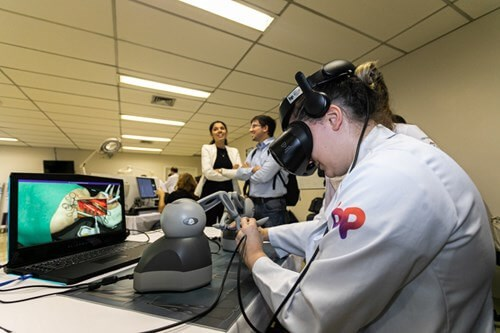
\includegraphics[scale=0.8]{Cirurgia RV.jpg}
    \caption{Treinamento de cirurgiões com RV \cite{cirurgioesRV}}
    \label{RVimg}
\end{figure}

\newpage

\section{Relevância}

\paragraph{} Na disciplina de Realidade Virtual o aluno aprende como programar para a GPU usando a linguagem CUDA (desenvolvida pela NVIDIA). Como a GPU possui vários núcleos, um ponto bastante trabalhado é em como paralelizar o processamento para que o algoritmo seja executado no maior número de threads possíveis com a mínima dependência entre elas. \cite{wikiRel}

\section{Relação Com Outras Disciplinas}

\paragraph{} A disciplina de Realidade Virtual possui duas disciplinas como pré-requisito, e são elas:

\begin{itemize}
    \item IF681 - Interfaces Usuario-Maquina
    \item IF687 - Introdução a Multimidia
\end{itemize}

\bibliographystyle{plain}
\bibliography{ref}

\end{document}
